\chapter{Electromagnetism}
\section{Fundamental Concepts}
\subsection{Charge, Current, Flux}
\begin{qt}
    \begin{center}
        Electric charge is conserved no matter how small our system is, even for elementary particle processes
    \end{center}
\end{qt}
\begin{qt}
    The total charge inside any volume $V$ is then given by the integral over the charge density:
    \begin{equation}
Q=\int_{V} d^{3} x \rho(\vec{x}, t)
\end{equation}
\end{qt}
Of course, \textbf{we can also use the charge density if there is only one charged object in our system.} In this case, the charge density is zero everywhere except at one specific point. Any integral over a region which contains the location of the object, yields simply the charge of the object. 
\begin{qt}
    Specifically, the charge density of a system with just one charged object located at $\vec{x}_{0}$ is
    \begin{equation}
\rho(\vec{x})=q \delta\left(\vec{x}-\vec{x}_{0}\right)
\end{equation}
\end{qt}
where $q$ is the charge of the object. Any integral over a region $V_{0}$ which contains $\vec{x}_{0}$ yields exactly $q,$ as it should be
$$
\begin{aligned}
\int_{V_{0}} d^{3} x \rho(\vec{x}, t) &=\int_{V_{0}} d^{3} x q \delta\left(\vec{x}-\vec{x}_{0}\right) \\
&=q \int_{V_{0}} d^{3} x \delta\left(\vec{x}-\vec{x}_{0}\right) \\
&=q
\end{aligned}
$$
\begin{qt}
    In electrodynamics, the \redp{the electric current} is defined as:
    \begin{equation}
I=\frac{d Q}{d t}
\end{equation}
\end{qt}
The correct tool to describe the flow of charges in three dimensions is called \textbf{\redp{current density}}. \bluep{A current density yields a vector at each point in space(i.e., vector space). The direction of the vector at a given point describes the direction of the flow. The length of the vector describes how much is flowing.}
\begin{qt}
    By introducing a vector $\vec{n}$ of unit length normal to a frame with area of $A$, we can calculate the current passing through the frame as:
    \begin{equation}
I \equiv \frac{\Delta Q}{\Delta t}=\rho_{0} A \vec{v}_{c} \cdot \vec{n}
\end{equation}
If we define \textbf{\redp{the electric current density}} as 
\begin{equation}
\vec{J} \equiv \rho_{0} \vec{v}_{c}
\end{equation}
we have
\begin{equation}
\vec{J} \cdot \vec{n} A=\rho_{0} \vec{v}_{c} \cdot \vec{n} A=I
\end{equation}
\end{qt}
In general, \textbf{the magnitude of the current density $|\vec{J}|$ at one specific point describes the amount of electric charge which passes per unit time through an infinitesimal surface element which is at right angles to the direction of the flow.} The direction of the charge density vector $\vec{J}$ encodes where the charges are flowing.

\begin{qt}
    If we want to know how much electric charge is flowing through a more complicated surface $S$, we have to calculate the \textbf{\redp{surface integral}}:
    \begin{equation}
I=\int_{S} \vec{J} \cdot \overrightarrow{d S}
\end{equation}
The total amount of charge passing through the surface $S$ during some time interval $\Delta t$ is then given by
\begin{equation}
\Delta Q=\Delta t \int_{S} \vec{J} \cdot \overrightarrow{d S}
\end{equation}
\end{qt}

\subsection{Electromagnetic Field}
An important feature of the electromagnetic field is that even a vector field is not sufficient and we need instead a tensor field. \textbf{The electromagnetic field tensor is an antisymmetric $(4 \times 4)$ matrix}
\begin{qt}
    \begin{equation}
F_{\mu \nu}(t, \vec{x})=\left(\begin{array}{cccc}
{0} & {F_{01}(t, \vec{x})} & {F_{02}(t, \vec{x})} & {F_{03}(t, \vec{x})} \\
{-F_{01}(t, \vec{x})} & {0} & {F_{12}(t, \vec{x})} & {F_{13}(t, \vec{x})} \\
{-F_{02}(t, \vec{x})} & {-F_{12}(t, \vec{x})} & {0} & {F_{23}(t, \vec{x})} \\
{-F_{03}(t, \vec{x})} & {-F_{13}(t, \vec{x})} & {-F_{23}(t, \vec{x})} & {0}
\end{array}\right)
\end{equation}
\redp{This tensor field, in some sense, assigns exactly two vectors to each point in space $\vec{x}$ at each point in time $t .$ }
\end{qt}
The vectors at each location represent the strength and direction of the electromagnetic field. It is conventional to introduce the electric vector field $\vec{E}(t, \vec{x})$ and the magnetic vector field $\vec{B}(t, \vec{x})$ and work with them, instead of with the electromagnetic tensor field $F_{\mu \nu}(t, \vec{x})$.
\begin{equation}
F_{\mu \nu}(t, \vec{x})\equiv\left(\begin{array}{cccc}
{0} & {-E_{1}(t, \vec{x}) / c} & {-E_{2}(t, \vec{x}) / c} & {-E_{3}(t, \vec{x}) / c} \\
{E_{1}(t, \vec{x}) / c} & {0} & {-B_{3}(t, \vec{x})} & {B_{2}(t, \vec{x})} \\
{E_{2}(t, \vec{x}) / c} & {B_{3}(t, \vec{x})} & {0} & {-B_{1}(t, \vec{x})} \\
{E_{3}(t, \vec{x}) / c} & {-B_{2}(t, \vec{x})} & {B_{1}(t, \vec{x})} & {0}
\end{array}\right)
\end{equation}
\bluep{Each of these two fields $\vec{E}(t, \vec{x})=\left(E_{1}(t, \vec{x}), E_{2}(t, \vec{x}), E_{3}(t, \vec{x})\right)^{T}$
and $\vec{B}(t, \vec{x})=\left(B_{1}(t, \vec{x}), B_{2}(t, \vec{x}), B_{3}(t, \vec{x})\right)^{T}$ assigns a vector to each point in space $\vec{x}$ at each point in time $t$}.

Unfortunately, the interpretation of the electric field $\vec{E}(t, \vec{x})$ and the magnetic field $\vec{B}(t, \vec{x})$ is not so simple. Instead, the little arrows encode information about the somewhat abstract "physical field", which we can understand as follows: \redp{The direction of the vector at a given location encodes in which direction a test charge would move if it were placed here. The magnitude of the vector encodes how fast the test charge would accelerate as a result of, for example, the electric field}. In this sense, these more abstract fields encode how something would
flow if it were there.
\begin{qt}
    In practice the electric field strength at a point is measured by placing a small test charge at that point and measuring the force on it:
    \begin{equation}
\vec{E}(\vec{x}) \equiv \frac{\vec{F}(\vec{x})}{q}
\end{equation}
\end{qt}
\subsection{Electromagnetic potential}
For the moment, we only note that the electromagnetic potential is characterized by 4 numbers at each point in space and time $A_{\mu}(t, \vec{x})=\left(A_{0}(t, \vec{x}), A_{1}(t, \vec{x}), A_{2}(t, \vec{x}), A_{3}(t, \vec{x})\right)^{T}$ and that the electric and magnetic fields can be calculated immediately once the electromagnetic potential is specified:
\begin{qt}
    \begin{equation}
\begin{aligned}
&E_{i}=\left(-\partial_{i} A_{0}-\partial_{0} A_{i}\right) / c\\
&B_{i}=\epsilon_{i j k} \partial_{j} A_{k}
\end{aligned}
\end{equation}
where $i, j, k \in\{1,2,3\} .$ We can also write this as a vector equations
\begin{equation}
\begin{aligned}
&\vec{E}=\left(-\nabla A_{0}-\partial_{t} \vec{A}\right) / c\\
&\vec{B}=\nabla \times \vec{A}
\end{aligned}
\end{equation}
\end{qt}
We can also express the tensor field itself using the electromagnetic potential
\begin{qt}
    \begin{equation}
F_{\mu v}=\partial_{\mu} A_{v}-\partial_{v} A_{\mu}
\end{equation}
\end{qt}

\section{Fundamental Equations}
The Lorentz force law describes how charged object react to the presence of the electric and magnetic field. Maxwell's equations describe how non-zero electric and magnetic field strengths are generated by charges and currents. Moreover, they also describe how the electric and magnetic fields influence each other. In addition, the continuity equation encodes the fact that electric charge is conserved. All this is summarized by the following diagram:
\begin{qt}
    \begin{center}
        


\tikzset{every picture/.style={line width=0.75pt}} %set default line width to 0.75pt        

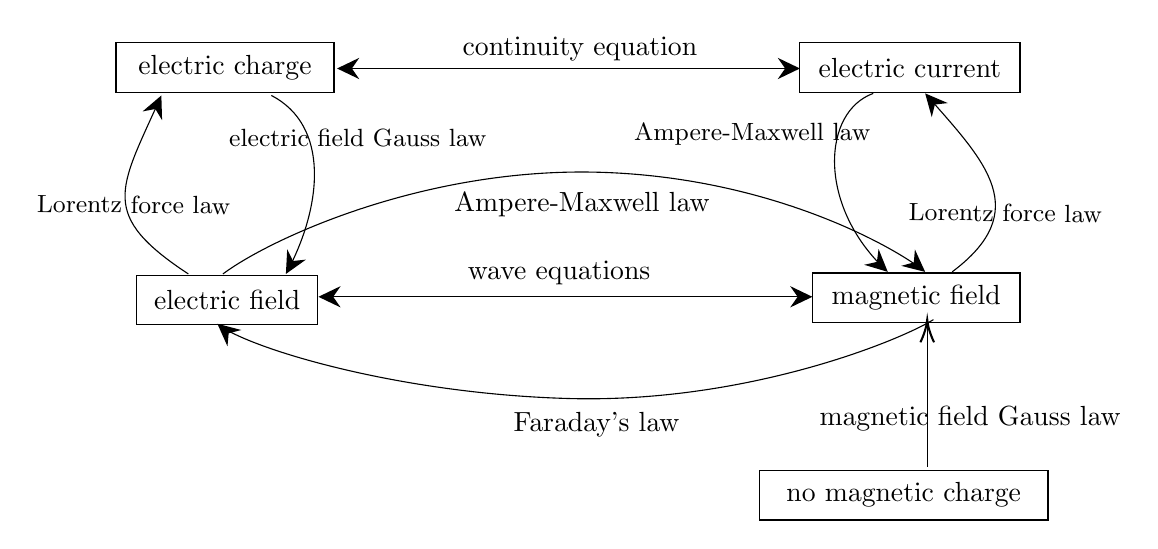
\begin{tikzpicture}[x=0.75pt,y=0.75pt,yscale=-1,xscale=1]
%uncomment if require: \path (0,300); %set diagram left start at 0, and has height of 300

%Straight Lines [id:da6043751763886723] 
\draw    (177,53.47) -- (394,53.47) ;
\draw [shift={(397,53.47)}, rotate = 180] [fill={rgb, 255:red, 0; green, 0; blue, 0 }  ][line width=0.08]  [draw opacity=0] (10.72,-5.15) -- (0,0) -- (10.72,5.15) -- (7.12,0) -- cycle    ;
\draw [shift={(174,53.47)}, rotate = 0] [fill={rgb, 255:red, 0; green, 0; blue, 0 }  ][line width=0.08]  [draw opacity=0] (10.72,-5.15) -- (0,0) -- (10.72,5.15) -- (7.12,0) -- cycle    ;
%Straight Lines [id:da07068797370513968] 
\draw    (168,163.47) -- (400,163.47) ;
\draw [shift={(403,163.47)}, rotate = 180] [fill={rgb, 255:red, 0; green, 0; blue, 0 }  ][line width=0.08]  [draw opacity=0] (10.72,-5.15) -- (0,0) -- (10.72,5.15) -- (7.12,0) -- cycle    ;
\draw [shift={(165,163.47)}, rotate = 0] [fill={rgb, 255:red, 0; green, 0; blue, 0 }  ][line width=0.08]  [draw opacity=0] (10.72,-5.15) -- (0,0) -- (10.72,5.15) -- (7.12,0) -- cycle    ;
%Curve Lines [id:da13680905709879954] 
\draw    (119,152.47) .. controls (141.6,135.52) and (216.12,101.05) .. (300.33,103.47) .. controls (380.34,105.76) and (438.25,137.2) .. (455.03,149.66) ;
\draw [shift={(457.33,151.47)}, rotate = 219.81] [fill={rgb, 255:red, 0; green, 0; blue, 0 }  ][line width=0.08]  [draw opacity=0] (10.72,-5.15) -- (0,0) -- (10.72,5.15) -- (7.12,0) -- cycle    ;

%Curve Lines [id:da32747829322015765] 
\draw    (119,178.38) .. controls (137.27,189.89) and (205.75,210.19) .. (285.33,212.47) .. controls (369.55,214.88) and (443.33,185.47) .. (461.33,174.47) ;

\draw [shift={(116.33,176.47)}, rotate = 40.24] [fill={rgb, 255:red, 0; green, 0; blue, 0 }  ][line width=0.08]  [draw opacity=0] (10.72,-5.15) -- (0,0) -- (10.72,5.15) -- (7.12,0) -- cycle    ;
%Straight Lines [id:da5861609067826448] 
\draw    (458.33,245.47) -- (458.33,176.47) ;
\draw [shift={(458.33,174.47)}, rotate = 450] [color={rgb, 255:red, 0; green, 0; blue, 0 }  ][line width=0.75]    (10.93,-3.29) .. controls (6.95,-1.4) and (3.31,-0.3) .. (0,0) .. controls (3.31,0.3) and (6.95,1.4) .. (10.93,3.29)   ;

%Curve Lines [id:da35984262406569245] 
\draw    (470.33,151.47) .. controls (509.53,122.07) and (486.31,98.43) .. (459.01,67.38) ;
\draw [shift={(457.33,65.47)}, rotate = 408.81] [fill={rgb, 255:red, 0; green, 0; blue, 0 }  ][line width=0.08]  [draw opacity=0] (10.72,-5.15) -- (0,0) -- (10.72,5.15) -- (7.12,0) -- cycle    ;

%Curve Lines [id:da050391804224369396] 
\draw    (432.33,65.47) .. controls (407.83,74.29) and (405.42,118.64) .. (437.34,149.59) ;
\draw [shift={(439.33,151.47)}, rotate = 222.36] [fill={rgb, 255:red, 0; green, 0; blue, 0 }  ][line width=0.08]  [draw opacity=0] (10.72,-5.15) -- (0,0) -- (10.72,5.15) -- (7.12,0) -- cycle    ;

%Curve Lines [id:da7848731503908734] 
\draw    (102.33,152.47) .. controls (59.21,124.05) and (68.92,111.95) .. (88.14,69.13) ;
\draw [shift={(89.33,66.47)}, rotate = 473.96] [fill={rgb, 255:red, 0; green, 0; blue, 0 }  ][line width=0.08]  [draw opacity=0] (10.72,-5.15) -- (0,0) -- (10.72,5.15) -- (7.12,0) -- cycle    ;

%Curve Lines [id:da2947796011268943] 
\draw    (142.33,66.47) .. controls (170.61,81.09) and (166.56,119.48) .. (150.59,150.13) ;
\draw [shift={(149.33,152.47)}, rotate = 298.74] [fill={rgb, 255:red, 0; green, 0; blue, 0 }  ][line width=0.08]  [draw opacity=0] (10.72,-5.15) -- (0,0) -- (10.72,5.15) -- (7.12,0) -- cycle    ;


% Text Node
\draw    (67.5,41) -- (172.5,41) -- (172.5,65) -- (67.5,65) -- cycle  ;
\draw (120,53) node   [align=left] {electric charge};
% Text Node
\draw    (397,41) -- (503,41) -- (503,65) -- (397,65) -- cycle  ;
\draw (450,53) node   [align=left] {electric current};
% Text Node
\draw    (77.5,153) -- (164.5,153) -- (164.5,177) -- (77.5,177) -- cycle  ;
\draw (121,165) node   [align=left] {electric field};
% Text Node
\draw    (403,152) -- (503,152) -- (503,176) -- (403,176) -- cycle  ;
\draw (453,164) node   [align=left] {magnetic field};
% Text Node
\draw    (377.5,247) -- (516.5,247) -- (516.5,271) -- (377.5,271) -- cycle  ;
\draw (447,259) node   [align=left] {no magnetic charge};
% Text Node
\draw (291,44) node   [align=left] {continuity equation};
% Text Node
\draw (281,152) node   [align=left] {wave equations};
% Text Node
\draw (292,119) node   [align=left] {Ampere-Maxwell law};
% Text Node
\draw (299,225) node   [align=left] {Faraday's law};
% Text Node
\draw (479,222) node   [align=left] {magnetic field Gauss law};
% Text Node
\draw (496,123) node  [font=\small,rotate=-0.65] [align=left] {Lorentz force law};
% Text Node
\draw (374,85) node  [font=\small] [align=left] {Ampere-Maxwell law};
% Text Node
\draw (184,87) node  [font=\small] [align=left] {electric field Gauss law};
% Text Node
\draw (76,119) node  [font=\small,rotate=-0.65] [align=left] {Lorentz force law};


\end{tikzpicture}

    \end{center}
\end{qt}
\subsection{Continuity equation}
\begin{qt}
    \begin{equation}
\frac{\partial}{\partial t} \int_{V} \rho d V=\oint_{S} \vec{J} \cdot \overrightarrow{d S}
\end{equation}
\end{qt}
The continuity equation really describes the local conservation of electric charge. In words, the continuity equation tells us: \bluep{the at which the charge density changes in a given volume is exactly equal to the net amount of electric charge flowing through the surface of the volume per unit time.}

Using Gauss's theorem, we have
\begin{equation}
\oint_{S} \vec{J} \cdot \overrightarrow{d S}=\int_{V} \nabla \cdot \vec{J} d V
\end{equation}
and we get the \textbf{differential form of the continuity equation}
\begin{qt}
    \begin{equation}
\frac{\partial}{\partial t} \rho-\nabla \cdot \vec{J}=0
\end{equation}
\end{qt}
\subsection{Lorentz force law}
\begin{qt}
    \begin{equation}
\vec{F}_{E}=q \vec{E}
\end{equation}
\begin{equation}
\vec{F}_{B}=q \vec{v} \times \vec{B}
\end{equation}
\end{qt}
The Lorentz force law consists of two parts. The first part, tells us that the force resulting from the electric field $\vec{E}$ is directly proportional to $\vec{E}$. The second part take into account that only moving charged objects react to the presence of the magnetic field. When the velocity $\vec{v}$ is completely perpendicular to the magnetic field $\vec{B}$, the trajectory is simply a circle.

The general Lorentz force law therefore reads
\begin{qt}
    \begin{equation}
\vec{F}=q(\vec{E}+\vec{v} \times \vec{B})
\end{equation}
\end{qt}

\subsection{Gauss's law for the electric field}
\textbf{\redp{Each electric charge generates a particular structure in the electromagnetic field and this, in turn, has a direct impact on other charges}}.

We first introduce the \textbf{flux of the electric field through some surface $S$}:
\begin{equation}
\phi \equiv \int_{S} \vec{E} \cdot \overrightarrow{d S}
\end{equation}
Our goal is to find an equation which describes that \textbf{a nonzero charge within some volume has a direct impact on the structure of the electric field}. The charge within some volume $V$ is given by $\int_{V} \rho d V$ and we just argued that \redp{\textbf{a reasonable object represent the electric field in such an equation is the flux of
the electric field}}:
\begin{qt}
    \begin{equation}
\oint_{S} \vec{E} \cdot \overrightarrow{d S}=\frac{1}{\epsilon_{0}} \int_{V} \rho d V
\end{equation}
\end{qt}
where $\epsilon_{0}$ is a constant known as \textbf{electric permittivity} which \textit{describes how strongly the electric field reacts to the presence of charges}. This is the integral form of Gauss's law for electric fields. In words, it tells us:
\begin{qt}
    The flux of the electric field passing through a closed surface is directly proportional to the amount of electric charge contained inside the surface.
\end{qt}
\bluep{Note that "flux" here is simply a statement about the \textbf{length of the vectors at the boundary of our volume.} Moreover, if the sign of the flux is positive, the vectors point outwards and \textit{vice versa}}.
\begin{qt}
    \begin{itemize}
        \item $\vec{J}$ and $\vec{E}$ assign a vector to each point in space.
        \item For $\vec{J}$ these vectors represent the real movement of our electric charges. For the more abstract electric field $\vec{E},$ the arrows only represent how a charge would move if it were there.
        
    \end{itemize}
\end{qt}

Using Gauss's theorem, we also have \textbf{the differential form of Gauss's law for the electric field}:
\begin{qt}
    \begin{equation}
\nabla \cdot \vec{E}=\frac{\rho}{\epsilon_{0}}
\end{equation}
\end{qt}
\textit{\textbf{In general, the divergence of a vector field gives us information about the tendency of the field to flow towards or away from a specific point.}} With this in mind, we can say that the differential form of Gauss’s law for the electric field tells us:
\begin{qt}
    The structure of the electric field generated by electric charges is such that it converges upon negative charges and diverges from positive charges.
\end{qt}
The integral form is especially useful for macroscopic problems
which posses a high degree of symmetry, e.g. when there is a rotationally symmetric charge distribution. The differential form is useful, for example, when we want to talk about electromagnetic waves.
\subsection{Gauss's law for the magnetic field}
So far no non-zero magnetic
charge density has ever been observed, and \textbf{the integral form of Gauss's law for the magnetic field} reads
\begin{qt}
    \begin{equation}
\oint_{S} \vec{B} \cdot \overrightarrow{d S}=0
\end{equation}
\end{qt}
Thus, this equation tells us
\begin{qt}
    The flux of the magnetic field passing through any closed surface is zero.
\end{qt}
Again, \textbf{the differential form is}
\begin{qt}
    \begin{equation}
\nabla \cdot \vec{B}=0
\end{equation}
Since the right-hand side of our equation is zero, we can conclude that\textbf{ the tendency of the magnetic field to flow towards a point P is always exactly equal to its tendency to flow away from P. Any "inflow" of the magnetic field is always accompanied by an "outflow" of exactly the same magnitude.}
\end{qt}
\bluep{If the divergence is non-zero, the structure was created by a fundamental charge. If the divergence is zero, the structure was created by a different field (or a current).}

The non-zero magnetic field strengths generated by conventional magnets are generated by the billions of individual electrons which exist inside any macroscopic object. \textbf{\bluep{Each electron orbits around a nucleus and possesses a non-zero internal angular momentum}}. The special thing about magnets is that in these objects \textbf{\bluep{the majority of electrons rotate around approximately the same axis}}.

Note that \textbf{\redp{we can also achieve a non-zero electric field with zero divergence.} This is described by Faraday's law. The structure of the electric field generated by a changing magnetic field circulates back on itself}.

\subsection{Faraday's law}
We want a description in which a non-zero electric field strength shows up when the magnetic field is changing. The correct mathematical notion this task are time-derivatives. If the time-derivative of the magnetic field is non-zero, this means that the magnetic field is changing over time. Hence, our first puzzle piece is
$$
\dots=\int_{S} \frac{\partial}{\partial t} \vec{B} \cdot \overrightarrow{d S}
$$
The second puzzle piece that we need is something which describes the structure of the electric field that results from such a changing magnetic field.

A first hint is that the left-hand side must depend on our choice of the surface $S$ too. However, a volume integral over $\vec{E}$ is not a good idea since then $S$ would represent the surface of the volume. As a result $S$ would be a closed surface and, as mentioned above, Gauss's law for the magnetic field tells us that the integral over the magnetic field for any closed surface vanishes. Thus we use the boundary of a surface:
\begin{qt}
    \begin{equation}
\oint_{\mathrm{C}} \vec{E} \cdot \overrightarrow{d l}=-\int_{S} \frac{\partial}{\partial t} \vec{B} \cdot \overrightarrow{d S}
\end{equation}
The contour integral of LHS describes the circulation of the electric field. The minus sign encodes in which direction the resulting electric field circulates.
\end{qt}
To summarize, Faraday's law tells us
\begin{qt}
    A changing magnetic field flux generates a circulating structure in the electric field.
\end{qt}
\begin{mybox}
What's the physical meaning of a contour integral like $\oint_{C} \vec{E} \cdot \overrightarrow{d l}$?
\end{mybox}
\begin{mybox2}
From Lorentz force laws, we have 
$$
\begin{aligned}
\oint_{C} \vec{E} \cdot \overrightarrow{d l} &=\oint_{C} \frac{\vec{F}}{q} \cdot \overrightarrow{d l} \\
&=\frac{1}{q} \oint_{C} \vec{F} \cdot \overrightarrow{d l} \\
& \equiv \frac{W}{q}
\end{aligned}
$$
where$W$ denotes the work done by the electric field if we move a test charge $q$ along the path $C$.

\textbf{Therefore, we can conclude that the circulation of the electric field represents the energy for each unit of charge moving along the contour C.}
\end{mybox2}
Here, \redp{we use Stokes' theorem to derive the differential form of Faraday's theorem.}
\begin{equation}
\oint_{C} \vec{E} \cdot \overrightarrow{d l}=\int_{S} \nabla \times \vec{E} \cdot \overrightarrow{d S}
\end{equation}
\begin{qt}
    \begin{equation}
\nabla \times \vec{E}=-\frac{\partial}{\partial t} \vec{B}
\end{equation}
\end{qt}
\subsection{Ampere-Maxwell law}
\bluep{The Ampere-Maxwell law describes how a changing electric field generates a non-zero magnetic field strength}.\textbf{A non-zero magnetic field strength can be generated through
a changing electric field. We can also generate a non-zero magnetic field strength using moving electric charge.} Thus the integral form of the Ampere-Maxwell law reads
\begin{qt}
    \begin{equation}
\oint_{C} \vec{B} \cdot \overrightarrow{d l}=\mu_{0}\left(I_{\mathrm{enc}}+\epsilon_{0} \int_{S} \frac{\partial}{\partial t} \vec{E} \cdot \overrightarrow{d S}\right)
\end{equation}
$\mu_{0}$ and $\epsilon_{0}$ are proportionality constants known as vacuum permeability and vaccum permittivity. Moreover, $I_{enc}$ denotes the electric current enclosed by the contour $C$.
\end{qt}
By using Stokes' theorem, we find
$$
\begin{aligned}
\oint_{C} \vec{B} \cdot \overrightarrow{d l} &=\mu_{0}\left(I_{\mathrm{enc}}+\epsilon_{0} \int_{S} \frac{\partial}{\partial t} \vec{E} \cdot \overrightarrow{d S}\right) \\
\int_{S} \nabla \times \vec{B} \cdot \overrightarrow{d S} &=\mu_{0}\left(I_{\mathrm{enc}}+\epsilon_{0} \int_{S} \frac{\partial}{\partial t} \vec{E} \cdot \overrightarrow{d S}\right) \\
\int_{S} \nabla \times \vec{B} \cdot \overrightarrow{d S} &=\mu_{0}\left(\int_{S} \overrightarrow{J} \overrightarrow{d S}+\epsilon_{0} \int_{S} \frac{\partial}{\partial t} \vec{E} \cdot \overrightarrow{d S}\right) \\
\int_{S} \nabla \times \vec{B} \cdot \overrightarrow{d S} &=\mu_{0} \int_{S}\left(\vec{J}+\epsilon_{0} \frac{\partial}{\partial t} \vec{E}\right) \cdot \overrightarrow{d S}
\end{aligned}
$$
And \textbf{the differential form of the Ampere-Maxwell law} becomes
\begin{qt}
\begin{equation}
\nabla \times \vec{B}=\mu_{0}\left(\vec{J}+\epsilon_{0} \frac{\partial}{\partial t} \vec{E}\right)
\end{equation}
\end{qt}

\subsection{The wave equations}
To derive the equation of motion for the electric field $\overrightarrow{E}$, we start by taking the curl on both sides of Faraday's law:
$$
\begin{aligned}
\nabla \times \vec{E} &=-\frac{\partial}{\partial t} \vec{B} \\
\nabla \times \nabla \times \vec{E} &=-\nabla \times \frac{\partial}{\partial t} \vec{B} \\
\nabla \times \nabla \times \vec{E} &=-\frac{\partial}{\partial t} \nabla \times \vec{B}
\end{aligned}
$$
Using the follwoing vector identity
\begin{qt}
\begin{equation}
\nabla \times \nabla \times \vec{E}=\nabla(\nabla \cdot \vec{E})-\nabla^{2} \vec{E}
\end{equation}
\end{qt}
We have:
$$
\begin{aligned}
\nabla \times \nabla \times \vec{E} &=-\frac{\partial}{\partial t} \nabla \times \vec{B} \\
\nabla(\nabla \cdot \vec{E})-\nabla^{2} \vec{E} &=-\frac{\partial}{\partial t} \nabla \times \vec{B} \\
\nabla(\nabla \cdot \vec{E})-\nabla^{2} \vec{E} &=-\frac{\partial}{\partial t}\left(\mu_{0}\left(\vec{J}+\epsilon_{0} \frac{\partial}{\partial t} \vec{E}\right)\right)
\end{aligned}
$$
Gauss's law for the electric field reads $\nabla \cdot \vec{E}=\frac{\rho}{\epsilon_{0}}$, we have
$$
\nabla\left(\frac{\rho}{\epsilon_{0}}\right)-\nabla^{2} \vec{E}=-\frac{\partial}{\partial t}\left(\mu_{0}\left(\vec{J}+\epsilon_{0} \frac{\partial}{\partial t} \vec{E}\right)\right)
$$
And finally, we obtain \textbf{the wave equation for the electric field}
\begin{qt}
\begin{equation}
\nabla^{2} \vec{E}=\mu_{0} \epsilon_{0} \frac{\partial^{2}}{\partial t^{2}} \vec{E}
\end{equation}
\end{qt}
By following completely analogues steps, we have
\textbf{the wave equation for the magnetic field} as
\begin{qt}
\begin{equation}
\nabla^{2} \vec{B}=\mu_{0} \epsilon_{0} \frac{\partial^{2}}{\partial t^{2}} \vec{B}
\end{equation}
\end{qt}

So in summary, 
static charged object $\rightarrow$ static radial electric field

moving charged object $\rightarrow$ static circulating magnetic field

changing magnetic field $\rightarrow$ changing circulating electric field 

changing electric field $\rightarrow$ changing circulating magnetic field.

\section{Eletrostatics and Magnetostatics}
If the charge density is static $\left(\partial_{t} \rho=0\right),$ the resulting electric field configuration is time-independent. Analogously, if our current is steady $\left(\partial_{t} \vec{J}=0\right),$ the resulting magnetic field configuration is time-independent.

\bluep{In such systems we can treat the electric field and the magnetic field independently} because only if the electric field is changing does it have an effect on the magnetic field and vice versa.

For the electric field, we have
\begin{qt}
\begin{equation}
\begin{aligned}
\nabla \cdot \vec{E} &=\frac{\rho}{\epsilon_{0}} \\
\nabla \times \vec{E} &=0
\end{aligned}
\label{electrostatic}
\end{equation}
\end{qt}
The general solution to the electrostatic equations in (\ref{electrostatic}) is known as \redp{Coulomb's law}
\begin{qt}
\begin{equation}
\vec{E}(\vec{r})=\frac{1}{4 \pi \epsilon_{0}} \int \frac{\rho(\vec{r})\left(\vec{r}-\vec{r}^{\prime}\right)}{\left|\vec{r}-\vec{r}^{\prime}\right|^{3}} d^{3} \vec{r}^{\prime}
\label{coulombLaw}
\end{equation}
If we writing our charge distribution in terms of individual charges
$$
\rho(\vec{r})=\sum_{i} q_{i} \delta\left(\vec{r}-\vec{r}_{i}\right)
$$
we have
$$
\vec{E}(\vec{r})=\frac{1}{4 \pi \epsilon_{0}} \int \frac{\rho(\vec{r})\left(\vec{r}-\vec{r}^{\prime}\right)}{\left|\vec{r}-\vec{r}^{\prime}\right|^{3}} d^{3} \vec{r}^{\prime}=\sum_{i} \frac{q_{i}}{4 \pi \epsilon_{0}} \frac{\vec{r}-\vec{r}_{i}}{\left|\vec{r}-\vec{r}_{i}\right|^{3}}
$$
\end{qt}
For the magnetic field
\begin{qt}
\begin{equation}
\begin{aligned}
\nabla \cdot \vec{B} &=0 \\
\nabla \times \vec{B} &=\mu_{0} \vec{J}
\end{aligned}
\end{equation}
The solution has form of
\begin{equation}
\vec{B}(\vec{r})=\frac{\mu_{0}}{4 \pi} \int \frac{\vec{J}\left(\vec{r}^{\prime}\right) \times\left(\vec{r}-\vec{r}^{\prime}\right)}{\left|\vec{r}-\vec{r}^{\prime}\right|^{3}} d^{3} r^{\prime}
\label{Biot-SavartLaw}
\end{equation}
This is known as \textbf{Biot-Savart law}. It tells us that the magnetic field configuration generated by a general current density is simply the sum over the field configurations generated by the individual moving charges:
$$
\vec{J}(\vec{r})=\sum_{i} q_{i} \delta\left(\vec{r}-\vec{r}_{i}\right) \vec{v}_{i}
$$
Putting this into \ref{Biot-SavartLaw}
$$
\vec{B}(\vec{r})=\sum_{i} \frac{\mu_{0} q_{i}}{4 \pi} \vec{v}_{i} \times \frac{\vec{r}-\vec{r}_{i}}{\left|\vec{r}-\vec{r}_{i}\right|^{3}}
$$
\end{qt}
\subsection{Electric field of a single point charge}
Single point charge $\rho(\vec{r})=q \delta(\vec{r})$, using Gauss's law
$$
\oint_{S} \vec{E} \cdot \overrightarrow{d S}=\frac{1}{\epsilon_{0}} \int_{V} \rho d V
$$
$$
\int_{S} \vec{E} \cdot \overrightarrow{d S}=\frac{q}{\epsilon_{0}} \underbrace{\int_{V} \delta(\vec{r}) d V}_{=1}
$$
$$
\int_{S} \vec{E} \cdot \overrightarrow{d S}=\frac{q}{\epsilon_{0}}
$$
$$
\int_{0}^{2 \pi} \int_{0}^{\pi} E \underbrace{\vec{e}_{r} \cdot \vec{e}_{r}} r^{2} \sin (\theta) d \theta d \phi=\frac{q}{\epsilon_{0}}
$$
Thus,
$$
E=\frac{q}{r^{2} 4 \pi \epsilon_{0}}
$$
And the \textbf{Coulomb potential} is 
\begin{qt}
\begin{equation}
\phi=\frac{Q q}{r 4 \pi \epsilon_{0}}
\label{coulombPotential}
\end{equation}
\end{qt}
\subsection{Electric field of a sphere}
charge distribution reads
$$
\rho(\vec{r})=\left\{\begin{array}{ll}
{\rho_{0},} & {\text { on the sphere: }|\vec{r}|=R} \\
{0,} & {\text { otherwise }}
\end{array}\right.
$$
Thus,
$$
\vec{E}(\vec{r})=0 \quad \text { for }|\vec{r}|<R
$$
and
$$
\vec{E}(\vec{r})=\frac{\rho_{0}}{4 \pi \epsilon_{0}} \int \frac{\delta\left(\left|\vec{r}^{\prime}\right|-R\right)\left(\vec{r}-\vec{r}^{\prime}\right)}{\left|\vec{r}-\vec{r}^{\prime}\right|^{3}} d^{3} r^{\prime}=\frac{\rho_{0}}{4 \pi \epsilon_{0}} \int_{0}^{2 \pi} \int_{0}^{\pi} \int_{0}^{\infty} \frac{\delta\left(\left|\vec{r}^{\prime}\right|-R\right)\left(\vec{r}-\vec{r}^{\prime}\right)}{\left|\vec{r}-\vec{r}^{\prime}\right|^{3}} r^{\prime 2} d r^{\prime} \sin (\theta) d \phi d \theta
$$
Thus, outside of the sphere the electric field is described by
$$
\vec{E}(\vec{r})=\frac{q}{4 \pi \epsilon_{0} r^{2}} \vec{e}_{r}
$$
\subsection{Electric field of an electric dipole}
For simplicity, we assume that we are dealing with two point charges and choose our coordinate system such that one charge sits at the origin. The charge density then reads
$$
\rho(\vec{x})=q \delta(\vec{x})-q \delta(\vec{x}-\vec{d})
$$
where $\vec{d}$ is a vector pointing from the charge at the origin to the second charge. We can now immediately write down the resulting electric field configuration because we know that we simply have to \textbf{use a superposition of the individual configurations}.
\begin{qt}
\begin{equation}
\vec{E}(r)=\vec{E}_{q}(r)+\vec{E}_{-q}(r)=\frac{q \vec{r}}{4 \pi \epsilon_{0}|\vec{r}|^{3}}-\frac{q(\vec{r}-\vec{d})}{4 \pi \epsilon_{0}|\vec{r}-\vec{d}|^{3}} \vec{e}_{r}
\end{equation}
\end{qt}
\subsection{Electric field of more complicated charge distributions}
The general formula for the electric potential is
\begin{equation}
\phi(\vec{r})=\frac{1}{4 \pi \epsilon_{0}} \int \frac{\rho\left(\vec{r}^{\prime}\right)}{\left|\vec{r}-\vec{r}^{\prime}\right|} d^{3} r^{\prime}
\label{generalElectricPotential}
\end{equation}
We assume that the charge distribution $\rho\left(\vec{r}^{\prime}\right)$ is localized within some region $V .$ In mathematical terms, being far away from our charge distribution then means $|\vec{r}| \gg\left|\vec{r}^{\prime}\right|$ for all $\vec{r}^{\prime}$ in $V$

The main idea is that \textbf{we can then use \redp{Taylor expansion to simplify the general formula (\ref{generalElectricPotential})}}. In particular, we need the expansion
\begin{equation}
\begin{aligned}
\frac{1}{\left|\vec{r}-\vec{r}^{\prime}\right|} &=\frac{1}{r}-\vec{r}^{\prime} \cdot \nabla \frac{1}{r}+\ldots \\
&=\frac{1}{r}+\vec{r}^{\prime} \cdot \frac{\vec{r}}{r^{3}}+\ldots
\end{aligned}
\end{equation}
and
\begin{equation}
\begin{aligned}
\phi(\vec{r})=& \frac{1}{4 \pi \epsilon_{0}} \int \rho\left(\vec{r}^{\prime}\right) \frac{1}{\left|\vec{r}-\vec{r}^{\prime}\right|} d^{3} r^{\prime} \\
=& \frac{1}{4 \pi \epsilon_{0}} \int \rho\left(\vec{r}^{\prime}\right)\left(\frac{1}{r}+\vec{r}^{\prime} \cdot \frac{\vec{r}}{r^{3}}+\ldots\right) d^{3} r^{\prime} \\
=& \frac{1}{4 \pi \epsilon_{0} r} \int \rho\left(\vec{r}^{\prime}\right) d^{3} r^{\prime} \\
&+\frac{1}{4 \pi \epsilon_{0} r^{3}} \int \rho\left(\vec{r}^{\prime}\right) \vec{r}^{\prime} \cdot \vec{r} d^{3} r^{\prime}+\ldots
\end{aligned}
\end{equation}
\bluep{If we are sufficiently far away}, we can approximate our general formula as
$$
\phi(\vec{r}) \approx \frac{q}{4 \pi \epsilon_{0} r}
$$
\bluep{If we look closely enough}, we should describe the potential using
$$
\phi(\vec{r}) \approx \frac{q}{4 \pi \epsilon_{0} r}+\frac{1}{4 \pi \epsilon_{0} r^{3}} \int \rho\left(\vec{r}^{\prime}\right) \vec{r}^{\prime} \cdot \vec{r} d^{3} r^{\prime}
$$
where we can define
\begin{qt}
the \textbf{dipole moment}
\begin{equation}
\vec{p} \equiv \int \rho\left(\vec{r}^{\prime}\right) \vec{r}^{\prime} d^{3} r^{\prime}
\label{dipoleMoment}
\end{equation}
And the potential then reads
$$
\phi(\vec{r}) \approx \frac{q}{4 \pi \epsilon_{0} r}+\frac{1}{4 \pi \epsilon_{0} r^{3}} \vec{p} \cdot \vec{r}
$$
\end{qt}
Analogously it’s possible to introduce additional quantities which characterize the higher order terms in the Taylor expansion.
For example,
$$
\phi(\vec{r}) \approx \frac{1}{4 \pi \epsilon_{0}}\left(\frac{q}{r}+\frac{\vec{p} \cdot \vec{r}}{r^{3}}+\sum_{i j} \frac{Q_{i j} r_{i} r_{j}}{2 r^{5}}\right)
$$
where we have
\begin{qt}
the quadrupole moment defined as
\begin{equation}
Q_{i j} \equiv \int_{V} \rho\left(\vec{r}^{\prime}\right)\left(3 r_{i}^{\prime} r_{j}^{\prime}-\delta_{i j} r^{\prime 2}\right) d^{3} r^{\prime}
\label{quadrupoleMoment}
\end{equation}
\end{qt}
\redp{This method of collecting step-by-step information about complicated charge distributions is known as \textbf{multipole expansion}.}

\subsection{Magnetic field of a wire}
